\section{Routages des Fonctions
}
\subsection{Interface Microprocesseur}

Après l'étape de \textbf{synthèse}, nous pouvons nous intéresser à l'assignation des ressources 
matérielles du système.\\
Pour cela, nous utilisons le logiciel \textbf{Vivado} (étant donné que les outils de HDL n'étaient 
pas disponibles le jour du TP), qui permet de générer un schéma RTL ainsi qu'une vue du routage 
associé à l'interface microprocesseur.
\newline

Dans un premier temps, Nous allons resynthétiser le design afin d'obtenir le schéma RTL.
Ce schéma, présenté ci-dessous, illustre les ressources logiques utilisées pour implémenter 
l'interface microprocesseur.
\newline

\resizebox{\textwidth}{!}{%
    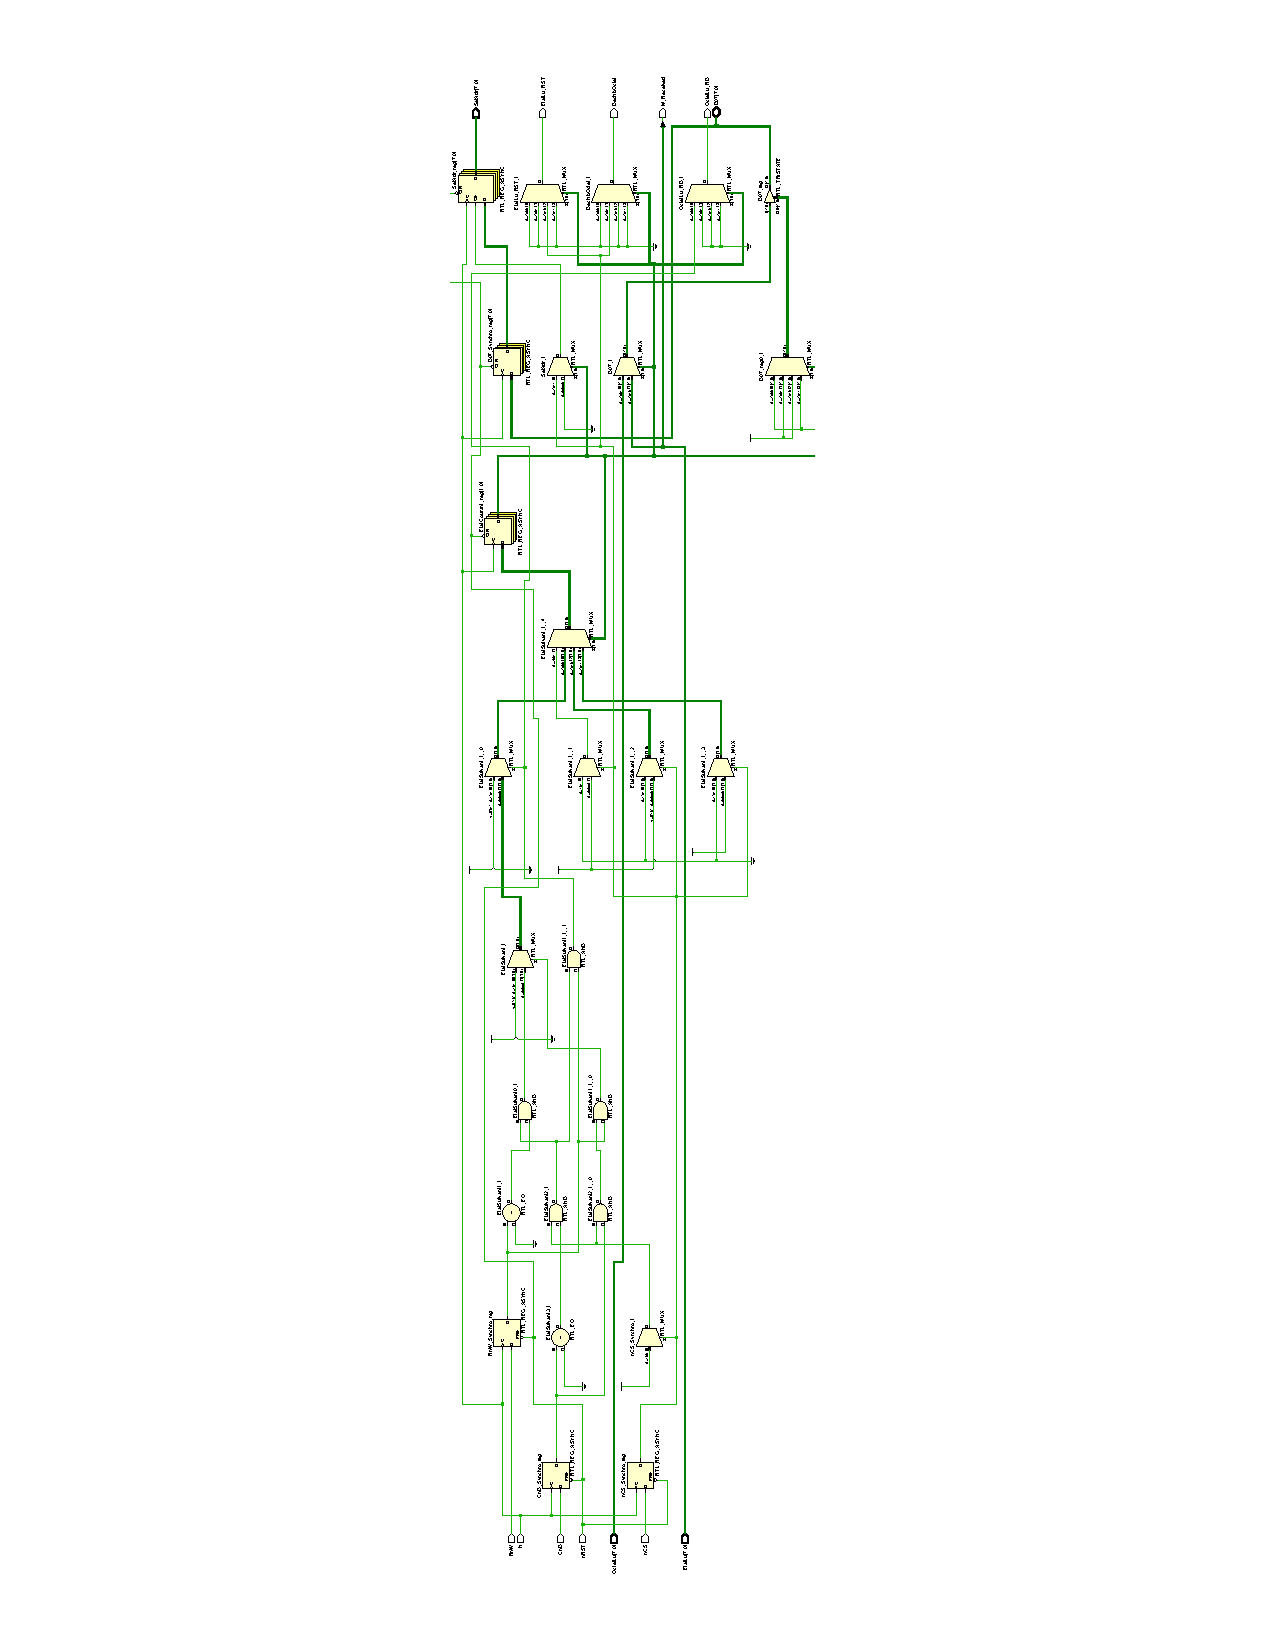
\includegraphics[angle=-90]{images/Routage/pdf_recadre_recadre.pdf}%
}

\vspace{10pt}

Par la suite, nous pouvons également observer la synthèse matérielle réalisée sur Vivado, qui 
transforme les ressources logiques en ressources matérielles pour le FPGA.
\newline

\begin{figure}[H]
    \centering
    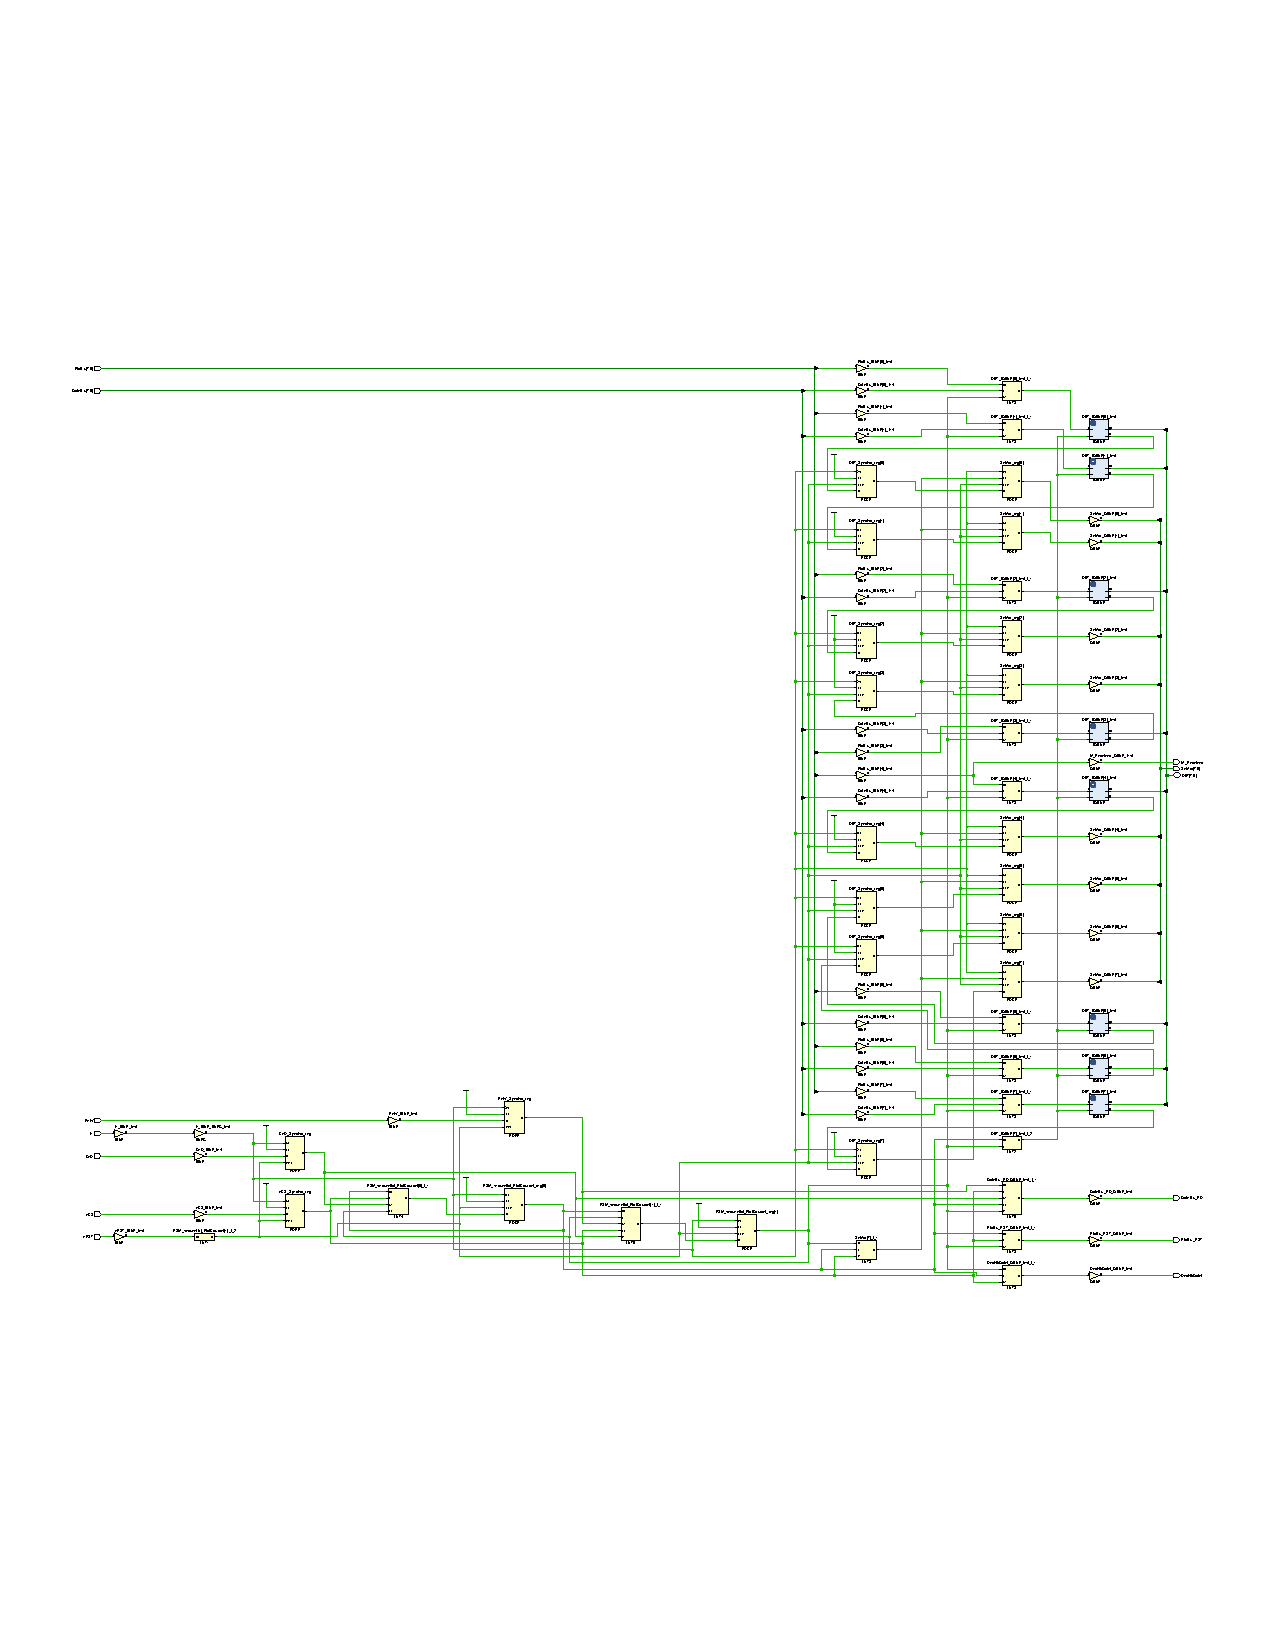
\includegraphics[width=0.8\linewidth]{images/Routage/schematic_RTL_VIVADO_recadre.pdf}
    \caption{Synthèse matérielle Vivado}
    \label{fig:rout_general}
\end{figure}

Cette synthèse nous montre que la logique est transformée en ressource matérielle, notamment des 
LUT (Look-Up Tables) et des Flip-Flops, qui sont les éléments de base pour implémenter la logique 
dans un FPGA.
\newline

Les \textbf{LUT} (Look-Up Tables), éléments fondamentaux d'un FPGA, peuvent être considérées comme 
des portes logiques programmables capables de réaliser toute fonction combinatoire. 
Elles constituent la base de l'implémentation matérielle et offrent une vision schématique complète 
du système.  
\newline

Prenons l'exemple d'une \textbf{LUT3} :  

\begin{figure}[H]
    \centering
    % Première image
    \begin{subfigure}[b]{0.55\linewidth}
        \centering
        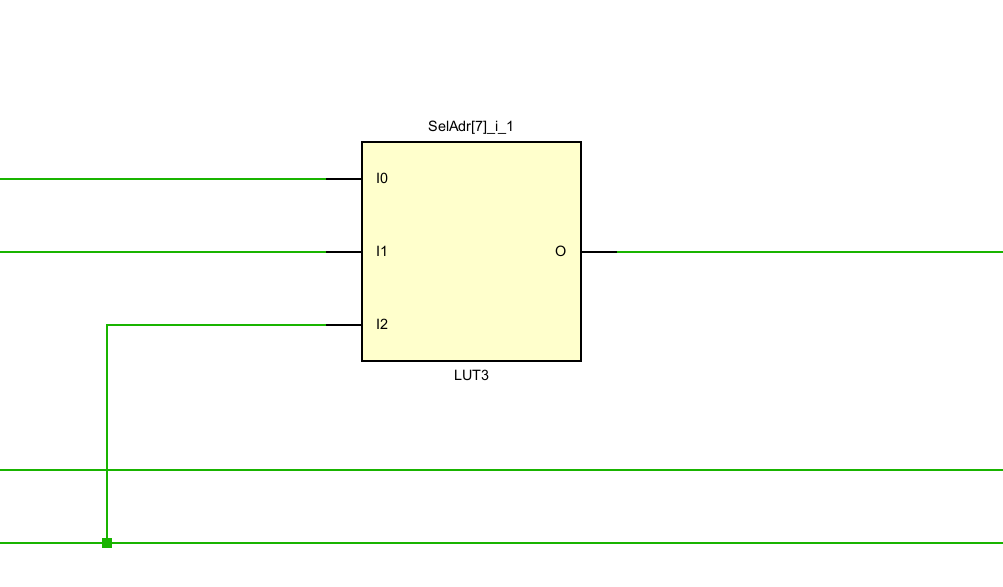
\includegraphics[width=\linewidth]{images/Routage/LUT_EXEMPLE.png}
        \caption{Exemple de LUT}
        \label{fig:lut_exemple}
    \end{subfigure}
    \hfill
    % Deuxième image
    \begin{subfigure}[b]{0.25\linewidth}
        \centering
        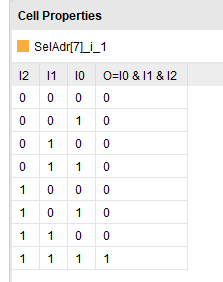
\includegraphics[width=\linewidth]{images/Routage/TABLE_LUT.png}
        \caption{Table de vérité associée}
        \label{fig:table_lut}
    \end{subfigure}
    \caption{Illustration d'une LUT et de sa table de vérité}
    \label{fig:lut_complete}
\end{figure}

Grace à la table de vérité de la LUT nous remarquons que cette LUT3 implémente une fonction logique ET à trois entrées.
\newline

\begin{figure}[H]
    \centering
    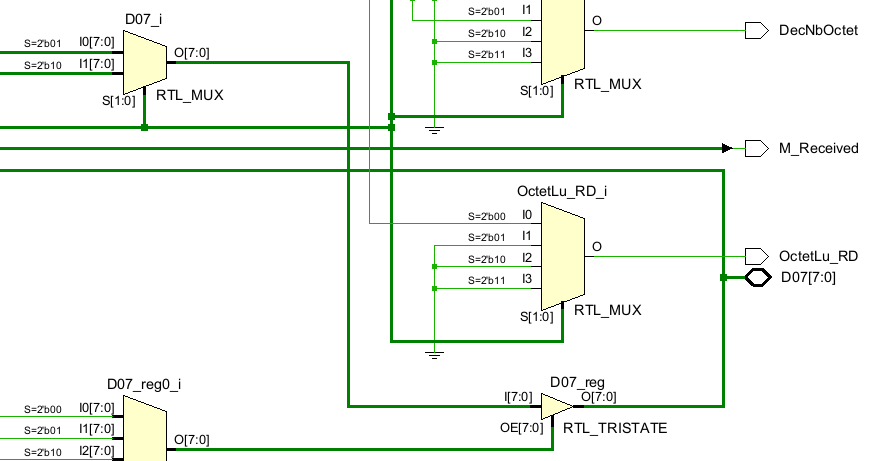
\includegraphics[width=0.8\linewidth]{images/Routage/Mux_Tris_Vivado.png}
    \caption{Synthèse Logique Vivado}
    \label{fig:rout_general}
\end{figure}

Nous observons également la présence de la partie opérative de l'interface Microprocesseur.
\newline

\medskip

La suite du flot de conception consiste à lancer l'\textbf{implémentation} du système afin d'obtenir le routage complet. 
Vivado propose alors une vue générale du FPGA, mettant en évidence ses différentes zones fonctionnelles :  

\begin{figure}[H]
    \centering
    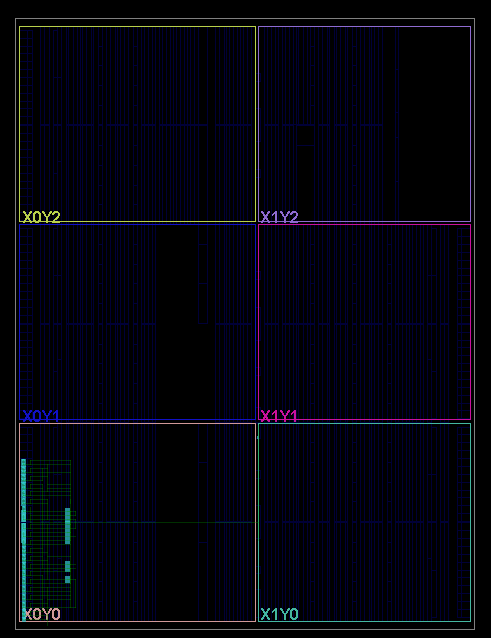
\includegraphics[width=0.8\linewidth]{images/Routage/Rout_1.png}
    \caption{Slice du FPGA après routage}
    \label{fig:rout_general}
\end{figure}

En effectuant un zoom, il est possible de constater que le système a été implémenté dans la zone \textbf{0} du FPGA. 
Nous observons que la zone située à gauche correspond aux entrées de chaque variable, 
celles-ci étant toutes reliées à des \textbf{buffers}.

\begin{figure}[H]
    \centering
    % Première image (anciennement deuxième)
    \begin{subfigure}[b]{0.45\linewidth}
        \centering
        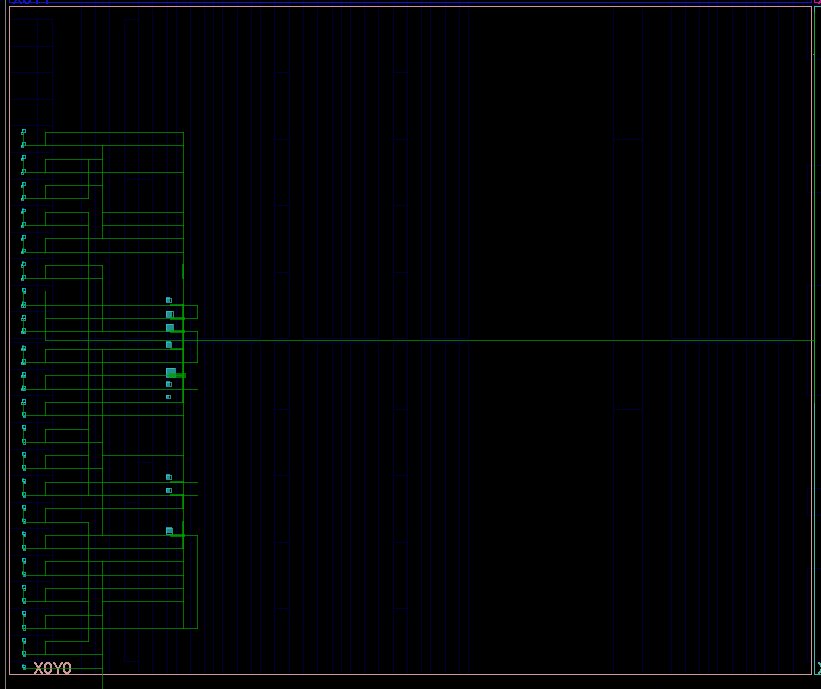
\includegraphics[width=\linewidth]{images/Routage/Rout_2.png}
        \caption{Localisation du système dans la zone 0 du FPGA}
        \label{fig:rout_zone0}
    \end{subfigure}
    \hfill
    % Deuxième image (anciennement première)
    \begin{subfigure}[b]{0.50\linewidth}
        \centering
        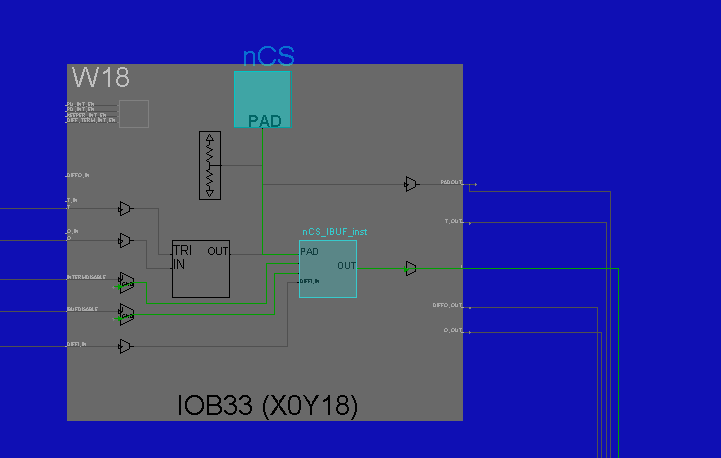
\includegraphics[width=\linewidth]{images/Routage/buff.png}
        \caption{Buffer associé à nCS}
        \label{fig:buff_ncs}
    \end{subfigure}
    \caption{Vue du système routé et des buffers associés sur le FPGA}
    \label{fig:rout_buff}
\end{figure}



Un zoom encore plus détaillé permet d'observer le câblage interne des ressources identifiées lors de la synthèse.  
Par exemple, une \textbf{LUT3} est câblée de la manière suivante :  

\begin{figure}[H]
    \centering
    % Première image
    \begin{subfigure}[b]{0.35\linewidth}
        \centering
        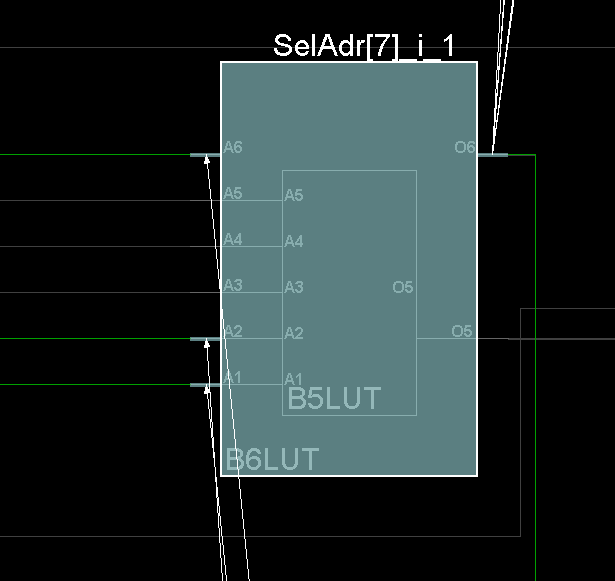
\includegraphics[width=\linewidth]{images/Routage/Rou_3.png}
        \caption{Connexion interne d'une LUT3}
        \label{fig:rout_lut3a}
    \end{subfigure}
    \hfill
    % Deuxième image
    \begin{subfigure}[b]{0.55\linewidth}
        \centering
        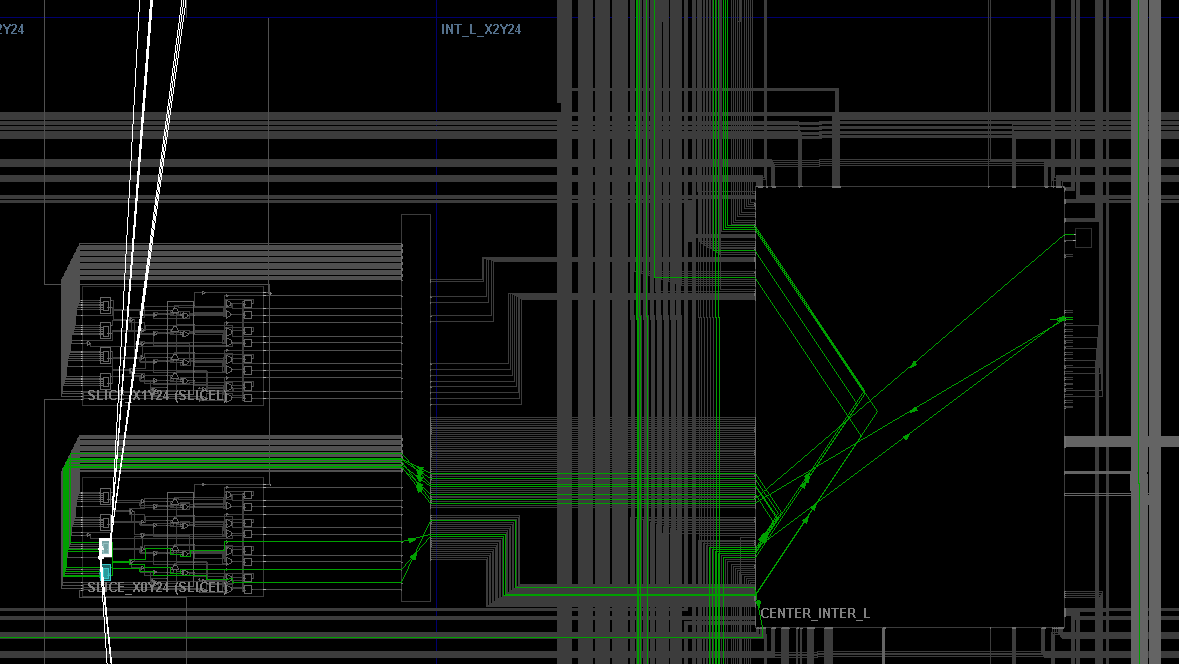
\includegraphics[width=\linewidth]{images/Routage/Rou_4.png}
        \caption{Schéma détaillé du câblage LUT3}
        \label{fig:rout_lut3b}
    \end{subfigure}
    \caption{Exemple de routage d'une LUT3 dans le FPGA}
    \label{fig:rout_lut3}
\end{figure}

\medskip

Le résultat final est une représentation complète et hiérarchisée du système, directement mappée sur le FPGA. 
\textbf{Vivado} offre ainsi la possibilité de visualiser l'ensemble du flot, depuis la description logique RTL jusqu'au routage physique détaillé.  

En résumé, la conception suit une progression en trois étapes :  
\begin{itemize}
    \item la \textbf{synthèse} génère une description logique optimisée du système (LUT, registres, blocs fonctionnels) ;  
    \item le \textbf{placement} attribue ces ressources aux cellules physiques du FPGA ;  
    \item le \textbf{routage} établit les interconnexions nécessaires au bon fonctionnement du circuit.  
\end{itemize}

Cette approche permet de passer d'une description abstraite en langage HDL à une implémentation matérielle 
concrète, où chaque fonction logique est traduite en ressources physiques. 
Vivado fournit alors une vision globale et détaillée du FPGA, allant de la logique combinatoire jusqu'au câblage interne des composants.
